\subsection{grep}
\emph{grep} är ett kommandotolkverktyg som används för att hitta textlinjer som matchar reguljära uttryck. 
\paragraph{Funktionalitet}
\emph{grep} tar emot ett reguljärt uttryck och söker sedan efter en linje som matchar och returnerar linjer med matchande delar upplyst. \emph{grep} kan konfigureras till att söka i olika medier som i en fil, input från användaren som unix pipes. Den kan även söka igenom kataloger efter filer vars namn matchar ett reguljärt uttryck och sedan kolla ifall den finner en matchning i dess innehåll.
\paragraph{Exempel: sökning i fil}
\begin{center}
        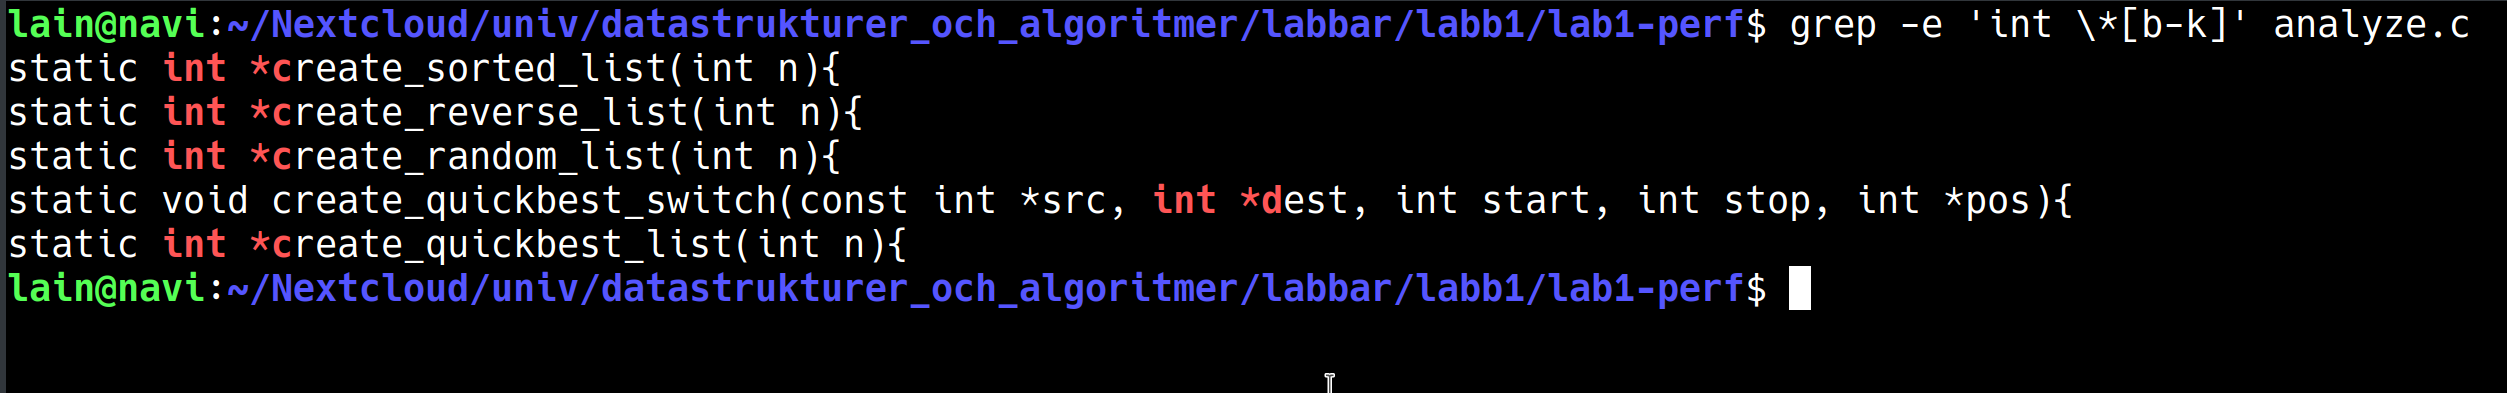
\includegraphics[width=\linewidth]{bilder/grep_sok_i_fil.png}
        \captionof{figure}{Sökning i fil}
\end{center}
Sökning i en c-fil efter linjer som innehåller deklarationer med int-pekare vars namn börjare med bokstäver i alfabetet från b till k.
\paragraph{Exempel: sökning i input}
\begin{center}
        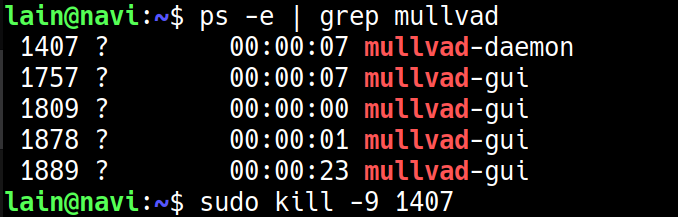
\includegraphics[width=\linewidth]{bilder/grep_pipes.png}
        \captionof{figure}{Sökning i input från annat program}
\end{center}
I exemplet tar \emph{grep} emot input från ett annat program för att hitta PID:en till en process med ett namn innehållandes mullvad. Kommandot ps -e har som output alla processer som körs på systemet som hade varit för mycket att söka igenom för hand.
\paragraph{Exempel: sökning efter fil med uttryck}
\begin{center}
        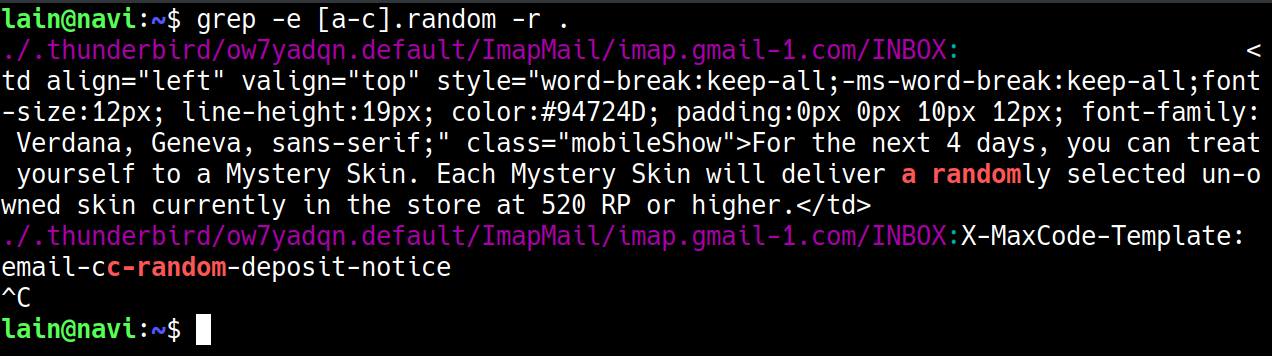
\includegraphics[width=\linewidth]{bilder/grep_sok_filer.png}
        \captionof{figure}{Sökning efter filer som har linjer som matchar uttryck}
\end{center}
\emph{grep} kan söka igenom en katalog efter filer vars innehåll matchar ett uttryck

